\chapter{Implementierung}
\label{cha:implementierung}

\section{Struktur}

Um eine modulare Implementierung der Software zu ermöglichen und darüber hinaus den Quellcode getrennt von nicht für die Öffentlichkeit bestimmten Daten (beispielsweise Anmeldedaten für APIs) bereitstellen zu können, ist es notwendig, die Softwareentwicklungsumgebung entsprechend zu gestalten. Die Unterteilung der für den Betrieb notwendigen Dateien inkl. des Quellcodes wird in den folgenden beiden Unterkapiteln beschrieben. Um die Lesbarkeit und Erweiterbarkeit zu verbessern, wurden die im Python Enhancement Proposal (PEP) Nr. 8\footnote{\url{https://peps.python.org/pep-0008/}} vorgeschlagenen Formatierungsrichtlinien umgesetzt. Sämtliche Module und Funktionen enthalten nach der Definition einen mehrzeiligen Kommentar mit einer Docstring-Dokumentation gemäß PEP 257\footnote{\url{https://peps.python.org/pep-0257/}} im Quellcode, siehe \autoref{lst:bsp-docstring}.

\begin{lstlisting}[caption={Beispiel für einen Docstring.}, label=lst:bsp-docstring, numbers=none]
def execute_query(query, seconds):
    """
    Diese Funktion führt eine ElasticSearch-Abfrage über die Graylog API aus.
    :param query: str, Graylog ElasticSearch-Abfrage
    :param seconds: int, Anzahl der Sekunden des relativen Zeitraums
    :return: Gibt die Anzahl der gezählten Ereignisse zurück
    """
\end{lstlisting}

Als Docstring wird ein mehrzeiliger Kommentar bezeichnet, welcher in der Zeile nach der Funktionsdefinition für den Entwickler wichtige Informationen enthält. Durch die standardisierte Syntax können die Informationen in vielen IDEs, darunter PyCharm von JetBrains, für eine interaktive Dokumentation innerhalb der Entwicklungsumgebung verwendet werden. Der Docstring enthält einen kurzen Satz zum funktionalen Umfang. Im Anschluss werden die Parameter und die von der Funktion zurückgegebenen Daten erläutert. Da Python dynamische Typisierung anwendet (Variablen werden nicht explizit mit einem Datentyp wie Ganzzahl oder Zeichenkette initialisiert sondern der Datentyp hängt vom zugewiesenen Wert ab), sorgen die Angaben für eine beschleunigte und, durch die Vermeidung von Typkonflikten, weniger fehleranfällige Entwicklung.

\subsection{Dateisystem}

Nachfolgend wird die Struktur der in \autoref{fig:dateisystem} dargestellten Ordner und Dateien erläutert.

\begin{figure}[h!]
\centering
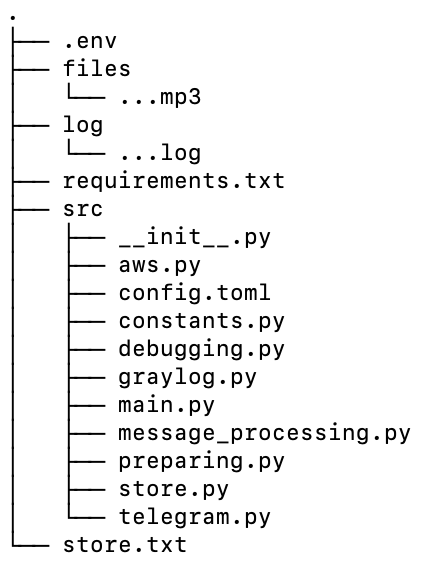
\includegraphics[scale=0.75]{dateisystem}
\caption{Gekürzte Ausgabe der für den Betrieb notwendigen Ordner und Dateien im Basisverzeichnis.}
\label{fig:dateisystem}
\end{figure}

\newpage

Von oben nach unten: 

\begin{itemize}
\item '.env' beinhaltet sensible Zugangsdaten für die verschiedenen Dienste und wird nicht in das öffentliche GitHub-Repository hochgeladen. 
\item 'files' dient als Zwischenspeicher für anfallende Audiodateien, welche aus den eingehenden Sprachnachrichten extrahiert wurden oder per Sprachsynthese erzeugt wurden. 
\item 'log' enthält die textbasierten Protokolle der Software. Zu jedem Start der Software wird eine neue Datei mit dem aktuellen Datum erzeugt. Die Inhalte der Dateien entsprechen der Konsolenausgabe mit der Ausnahme, dass sensible Daten nur in der Konsolenausgabe ausgegeben werden. 
\item requirements.txt dient als Informationsquelle für den Paketmanager Pip, mit welchem die Abhängigkeiten aus dem Python Package Index installiert werden können. Die Datei beinhaltet Namen und Versionsnummern von externen Softwaremodulen. 
\item 'src' beinhaltet Dateien mit dem Quellcode. 
\item '\_\_init\_\_.py' ist notwendig für die Moduldefinitionen in Python und hat keinen Inhalt 
\item 'store.txt' wird für die Persistierung des Werts für den Parameter 'update\_id' der Telegram Bot API verwendet.\cite[S. 337]{python}.

Weitere Dateien im Quellcode-Verzeichnis entsprechen den Modulen und werden im folgenden \autoref{sec:module} detaillierter erläutert. 

\end{itemize}

\enlargethispage{0.5cm} 

\subsection{Module}
\label{sec:module}

Der Quellcode wurde in mehrere Module aufgeteilt:

\begin{itemize}
\item \lstinline{main}: enthält die Hauptfunktion des Programms und startet die Vorbereitung und den Übergang in den Regelbetrieb.
\item \lstinline{debugging}: enthält die für die Fehlersuche notwendigen Funktionen. Siehe \autoref{sec:protokollierung}.
\item \lstinline{preparing}: enthält die für den Startvorgang notwendigen Funktionen, welche nicht Teil eines anderen Moduls sind. Siehe \autoref{sec:startvorgang}.
\item \lstinline{telegram}: enthält Funktionen für den Zugriff auf die Telegram-API. Die HTTP-Abfragen werden mit der Programmbibliothek \lstinline{requests}\footnote{\url{https://pypi.org/project/requests/}} durchgeführt. Weiterhin sind Funktionen für die Bearbeitung der Antworten der API enthalten. Die Authentifizierung an der API erfolgt über nur dem Entwickler bekannte Zugriffsschlüssel, welche vom Telegram-Bot \lstinline{@BotFather} ausgestellt werden.
\item \lstinline{aws}: enthält Funktionen für den Zugriff auf AWS. Für die Kommunikation mit der API wird boto3, das vom AWS-Team für Python bereitgestellte SDK, verwendet.
\item \lstinline{constants}: beinhaltet Konstanten, mit welchen der Ablauf des Programms gesteuert werden kann (beispielsweise können detaillierte Meldungen zum Programmablauf aktiviert oder bestimmte Telegram-Benutzer für den Zugriff auf den Bot autorisiert werden). Des Weiteren sind Variablen als Platzhalter Teil des Moduls, welche zur Laufzeit mit konstanten Objektdefinitionen der Boto3-Bibliothek überschrieben werden. Die Objektdefinitionen ermöglichen einen abstrakten Zugriff auf die AWS API, beispielsweise ohne notwendige erneute Authentifizierungen (dies übernimmt Boto3 im Hintergrund).
\item \lstinline{graylog}: beinhaltet Funktionen für den Zugriff auf die Graylog API. Der Zugriff erfolgt ähnlich wie beim Modul \lstinline{telegram} mit der Programmbibliothek \lstinline{requests}. Aus Sicherheitsgründen werden verschiedene Zugangsschlüssel für die Autorisierung und Authentifizierung verwendet\footnote{\url{https://docs.graylog.org/docs/rest-api}}. Der Access Token (dt. Zugriffsschlüssel) entspricht den Anmeldedaten an der Graylog Webschnittstelle und ermöglicht einen dauerhaften Zugriff. Mit dem Access token können zeitlich befristete Session Tokens (dt. Sitzungsschlüssel) generiert werden. Die Software erkennt anhand der von der API zurückgegebenen Fehlermeldung automatisch, wenn ein nicht gültiger Session Token verwendet wurde, und beantragt in diesem Fall einen neuen.
\item \lstinline{message_processing}: enthält interne Funktionen, welche für die Verarbeitung der erhaltenen Nachrichtentexte vorgesehen sind. 
\item \lstinline{store}: enthält Funktionen, welche für die Persistierung von Informationen notwendig sind. Die Telegram-API verwendet einen Zähler, welcher für jede Aktualisierung um einen Schritt inkrementiert wird. Ruft der Client Aktualisierungen von der API ab, erhält er den derzeitigen Stand als Wert der Variable 'update\_id' (vgl. fünfte Zeile aus \autoref{lst:bsp-telegram-api}). Bei weiteren Anfragen an die API gibt der Client die Variable 'update\_id' an, um nur Aktualisierungen zu erhalten, die seit der letzten Abfrage eingetroffen sind (und daher einen höheren Wert der Variable 'update\_id' haben). Die Variable 'update\_id' wird nach jeder Abfrage in die Textdatei store.txt auf das lokale Dateisystem geschrieben.
\end{itemize}

\section{Protokollierung}
\label{sec:protokollierung}

Für die Protokollierung wurde ein bereits vorhandenes, vom Autor dieser Arbeit entwickeltes Programmmodul erweitert, das Modul 'debugging' des GitHub-Repositorys 'Jomibe/wireguard-config-generator'\footnote{\url{https://github.com/Jomibe/wireguard-config-generator/blob/main/src/debugging.py}}. Das Repository enthält den Quellcode sowie die Dokumentation eines Softwareprojekts, welches im Rahmen des Moduls 'Projekt' im Sommersemester 2022 an der Fachhochschule Südwestfalen implementiert wurde. Es wurde eine Software entwickelt, mit welcher die Konfigurationsdateien eines WireGuard-VPN-Servers verwaltet werden können. Das Programm ermöglicht es unter anderem, die existierenden Konfigurationsdateien auf Syntax- und semantische Fehler zu prüfen und Konfigurationen für weitere VPN-Clients inkl. der Bestimmung von geeigneten Netzwerkkonfigurationen hinzuzufügen. Das Modul 'debugging' enthält Funktionen, welche für die Fehlersuche während der Laufzeit verwendet werden. In dem Modul wird die Funktion \lstinline{console()} implementiert, um die Ausgabe von Statusmeldungen auf der Konsole zentral zu koordinieren. 

Alle Statusmeldungen werden in einer Textdatei hinterlegt, deren Pfad in der Datei 'config.py' konfiguriert wird. Ist der \lstinline{DEBUG}-Modus aktiv, erscheinen alle Meldungen zusätzlich auf der Konsole. Ist die Fehlermeldung mit dem Parameter \lstinline{secret} gekennzeichnet, erfolgt keine Protokollierung in der Textdatei. Werden Meldungen auf der Konsole ausgegeben, werden diese gemäß dem Schweregrad farblich markiert. Dazu wird das die Programmbibliothek Colorama\footnote{\url{https://pypi.org/project/colorama/}} verwendet.

Bei der Formulierung der Fehlermeldungen wurden einige Anforderungen beachtet \cite[S. 495]{ux}: 

\begin{itemize}
\item Details zu fehlenden Informationen und Hinweise, wie diese Informationen übermittelt werden können. In diesem Anwendungsfall werden beispielsweise die Schlüsselwörter für Produktkategorien, Eigenschaften und Zeiträume genannt, wenn Informationen dazu fehlen.
\item Vermeidung von für den Anwender unverständliche technische Ausdrücken in den Fehlermeldungen.
\item Fehlermeldungen müssen den Benutzer möglichst schnell auf die Fehlerursache hinweisen und dürfen nicht vorwurfsvoll formuliert sein.
\end{itemize}

In \autoref{fig:bsp-err-log} und \autoref{fig:bsp-warn-log} ist die farbige Darstellung in der Konsole zu sehen. Im Anhang befinden sich zwei Listings mit ausführlicheren Konsolenausgaben, welche im folgenden Absatz erläutert werden.

\begin{figure}[h!]
\centering
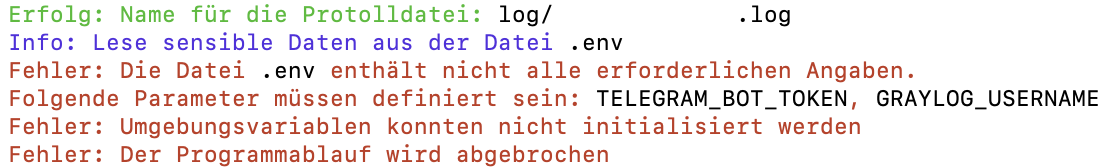
\includegraphics[scale=0.75]{bsp-err-log}
\caption{Farbige Ausgaben mit Fehlermeldungen.}
\label{fig:bsp-err-log}
\end{figure}

\begin{figure}[h!]
\centering
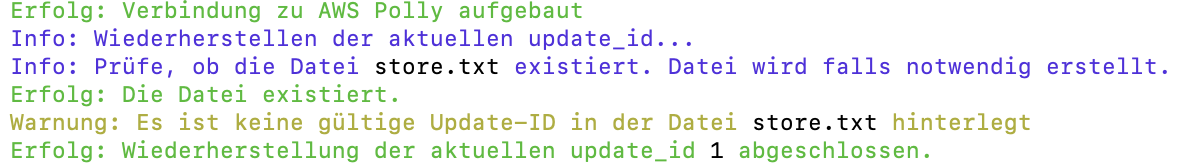
\includegraphics[scale=0.75]{bsp-warn-log}
\caption{Farbige Ausgaben mit Warnmeldungen.}
\label{fig:bsp-warn-log}
\end{figure}

\autoref{log-start}) zeigt die Konsolenausgabe während des Startvorgangs. Zu Beginn wird die Protokollierung in eine Textdatei initialisiert. Danach werden sensible Informationen wie Zugangsdaten aus der Datei .env in Umgebungsvariablen übernommen. Im Anschluss wird die Erreichbarkeit der Dienste von Telegram, Graylog und AWS geprüft. Schließlich wird die Konfiguration aus der Datei config.toml in eine interne Datenstruktur geladen, in welcher die Aliasdefinitionen (diese Funktion wird im \hyperref{ersten Unterkapitel des Abschnitts 4.4.2}[sec:aliasdef] beschrieben) aufgelöst werden. 

(\autoref{log-msg}) zeigt die Konsolenausgabe beim Verarbeiten einer eingegangenen Sprachnachricht. Im ersten Schritt wird der Zähler der Variable \lstinline{update_id} erhöht. Danach wird die Audiodatei von der Telegram Bot API bezogen, auf dem lokalen Dateisystem gespeichert und zu AWS Transcribe übertragen. Nachdem der Übertragungsprozess abgeschlossen ist, werden die Zwischenergebnisse der Transkription angezeigt. Ist der Transkriptionsprozess abgeschlossen, wird der Benutzer über den Status informiert und die Nachricht wird, nun in Textform, auf Schlüsselwörter analysiert. Anhand der Schlüsselwörter werden die Informationen extrahiert und mit den Werten aus der beim Start gefüllten Datenstruktur verglichen. Es wurde eine Übereinstimmung gefunden, somit kann eine Anfrage an Graylog gestellt werden. Das Ergebnis wird dem Benutzer mitgeteilt. Die Verarbeitung ist abgeschlossen und das Programm beginnt erneut mit dem Long-polling der Telegram Bot API.

\section{Startvorgang}
\label{sec:startvorgang}

Das Modul \lstinline{main} enthält die Methode \lstinline{main()}, welche den Startpunkt des Programms darstellt. In der Vorbereitungsphase (vgl. \autoref{sec:grundsaetzlicher-aufbau}) wird zuerst die Programmbibliothek \lstinline{colorama} initialisiert. Dies ist notwendig, um die Steuerung der Farbausgabe auf der Konsole an das zur Laufzeit verwendete Betriebssystem anzupassen\footnote{\url{https://github.com/tartley/colorama\#initialisation}}. Nach der Initialisierung wird die Funktion \lstinline{prepare()} aus dem Modul \lstinline{preparing} aufgerufen. Die Funktion besteht aus weiteren Funktionsaufrufen, welche jeweils mit einer positiven Rückmeldung abgeschlossen werden müssen. Wird eine Prüfung nicht erfolgreich abgeschlossen, gibt \lstinline{prepare()} den Wert \lstinline{False} zurück, und der Programmablauf wird nach Ausgabe einer detaillierten Fehlermeldung abgebrochen. Falls kein Fehlerstatus zurückgegeben wird, wird zum Regelbetrieb übergegangen. Dieser besteht aus einer Endlosschleife, in welcher die Funktion \lstinline{check_updates()} des Moduls \lstinline{telegram} aufgerufen wird.

\section{Regelbetrieb}

Im Regelbetrieb wird durch die Hauptfunktion in einer Endlosschleife die Funktion \lstinline{getUpdates()} aufgerufen (siehe \autoref{lst:code-main}). Diese führt Long-Polling der API-Funktion \lstinline{getUpdates} durch (siehe \autoref{lst:code-updates}). Eingehende Nachrichten werden in Echtzeit erkannt und weiterverarbeitet. Falls mehrere Nachrichten vorliegen (dies kommt vor, wenn die Software für längere Zeit nicht mit der Telegram-API verbunden war und in der Zwischenzeit mehrere Nachrichten an den Bot gesendet wurden), wird jeweils nur eine Nachricht verarbeitet, da die Variable 'update\_id' nur um jeweils einen Schritt (statt um die Anzahl der neuen Nachrichten) inkrementiert wird. Der Wert für den Ablauf der HTTP-Anfrage sollte so hoch wie möglich, aber so gering wie notwendig gewählt werden. Um Probleme durch Netzwerkinfrastruktur und Serverprozesse zu vermeiden, beträgt dieser standardmäßig 30 Sekunden \cite[Abs. 5.5. Timeouts]{rfc6202} und kann mittels des Parameters \lstinline{TELEGRAM_LONG_POLL_TIMEOUT} verändert werden. Dieser Parameter beeinflusst, wie lange die Verbindung seitens des Clients (diese Rolle übernimmt hier die in dieser Arbeit entwickelte Software) geöffnet bleibt. Nachdem die Zeit vergangen ist, wird die Anfrage mit einem Timeout vom Client abgebrochen. Durch die Endlosschleife wird sofort eine neue Anfrage gestartet. Trifft eine Antwort des Servers vor Ablauf der Zeitspanne ein, wird die Nachricht verarbeitet und die Software eröffnet im Anschluss eine neue Anfrage mit der angegebenen Wartezeit. Dies wird in \autoref{fig:long-polling} dargestellt. Der Ablauf der Verarbeitung wird im folgenden Absatz beschrieben.

\begin{lstlisting}[caption={Programmcode der Hauptfunktion ohne Kommentare und Ausgaben zur Fehleranalyse}, label=lst:code-main, numbers=none]
def main():
    colorama.init()
    if not prepare():
        console("Der Programmablauf wird abgebrochen", mode=ERR)
        return 1

    while True:
        check_updates()
\end{lstlisting}

\begin{lstlisting}[caption={Programmcode der Funktion für den Abruf von Aktualisierungen von der Telegram Bot API ohne Kommentare und Ausgaben zur Fehleranalyse}, label=lst:code-updates, numbers=none]
def get_updates():
    r = requests.get(url=f'https://api.telegram.org/bot{constants.telegram_bot_token}/getUpdates',
                     params={"offset": constants.telegram_update_id + 1,
                             "timeout": f"{TELEGRAM_LONG_POLL_TIMEOUT}",
                             "allowed_updates": '["message"]'
                             })
    if r.status_code == 200:
        console("Antwort in", f"{r.elapsed.microseconds/1000}ms", "erhalten", mode=SUCC)
    else:
        console("Telegram API ist nicht erreichbar. Details:", f"{r.status_code} {r.reason} - {r.text}", mode=ERR)
        return None
    return json.loads(r.text)
\end{lstlisting}

\begin{figure}[h!]
\centering
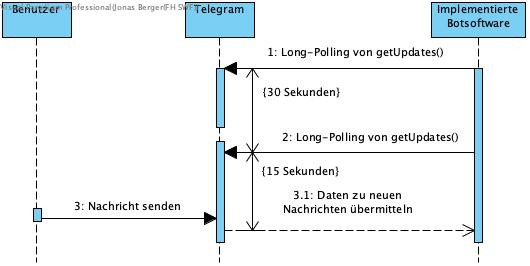
\includegraphics[scale=0.75]{long-polling}
\caption{Darstellung des zeitlichen Ablaufs des Long-pollings. Die erste Nachricht tritt 45 Sekunden nach Programmstart ein.}
\label{fig:long-polling}
\end{figure}

Zuerst wird anhand der Chat ID (vgl. Zeile 16 in \autoref{lst:bsp-telegram-api}) ermittelt, ob der Benutzer durch den Administrator für die Verwendung des Bots freigegeben wurde. Hierzu wird der Wert mit der Liste \lstinline{constants.AUTHORIZED_CHAT_IDS} verglichen. Bei positivem Ergebnis erfolgt die Verarbeitung der Nachrichteninhalte: Anhand des Aufbaus des JSON-Objekts wird ermittelt, ob es sich um eine Text- oder Sprachnachricht handelt. Der Text einer Nachricht wird direkt durch die Funktion \lstinline{message_processing.process_text_message} verarbeitet. Handelt es sich um eine Sprachnachricht, wird zuerst die Audiodatei von der Telegram Bot-API bezogen und auf dem lokalen Dateisystem abgelegt. Danach erfolgt der Transkriptionsprozess in einer weiteren Funktion, welche den ermittelten Text in einer Zeichenkette zurückgibt. Schließlich wird der Text ebenfalls durch die Funktion \lstinline{message_processing.process_text_message} verarbeitet.

\subsection{Optimierung der Antwortzeit}

Die Bedienung eines Systems mittels Sprache erfordert eine umfangreichere Benutzerführung als die Bedienung eines textbasierten Systems über einen Bildschirm und eine Tastatur. Beim Aufruf einer Webseite bietet der Bildschirm durch die Anzeige des Webbrowsers mit diversen Statuselementen eine dauerhafte Möglichkeit für den Benutzer, zu prüfen, ob die gewünschte Anfrage eingegangen ist und verarbeitet wird. Eine nur auf Sprache basierende Bedienung bietet keine äquivalente Möglichkeit, dem Benutzer eine Statusübersicht bis zum Abschluss der Anfrage zur Verfügung zu stellen. Um Missverständnisse vorzubeugen und die Bedienung komfortabel zu gestalten, muss das System eine Rückmeldung innerhalb eines durch den Menschen als nicht zu lang empfundenen Zeitraums zurückgeben. Dazu sollte die Zeit ohne sichtbare Veränderung eine Dauer von 10 Sekunden nicht überschreiten \cite[Kapitel 5.5]{response-time}\footnote{Auszug aus dem Buch: \url{https://www.nngroup.com/articles/response-times-3-important-limits/}}. 

Beim Test eines frühen Prototyps fiel auf, dass die Dauer zwischen Absenden der Sprachnachricht und Erhalt einer Antwort mit den Ergebnissen bis zu 30 Sekunden betrug. Diese Antwortzeit entspricht nicht dem oben genannten Richtwert von 10 Sekunden. Eine Analyse des Programmablaufs ergab, dass die Transkription und die Sprachsynthese (der Text-To-Speech Prozess) einen Großteil der benötigten Antwortzeit verursachten. Beide Prozesse wurden optimiert, die Optimierungen werden in den beiden folgenden Abschnitten beschrieben.

\subsubsection{Transkription}
\label{sec:optimierung-transk}

Ursprünglich wurde die Boto3-Bibliothek für die Interaktion mit Amazon Transcribe verwendet. Mit der Boto3-Bibliothek ist eine Verarbeitung in Echtzeit nicht möglich; die Audiodatei muss zuerst in einen S3-Speicher hochgeladen werden. Eine Möglichkeit für die direkte Zuführung der Datei besteht nicht. Im Anschluss muss ein Auftrag in Amazon Transcribe über das \lstinline{client}-Objekt in \lstinline{constants.aws_transcribe_obj} erstellt und die Datei im S3-Speicher damit verknüpft werden. Danach wird der Auftrag durch AWS verarbeitet. Die Möglichkeit eines Callbacks oder der Verwendung von Long-polling (vgl. \autoref{sec:telegram-getting-updates}) besteht nicht, daher muss die AWS-API mittels Polling durchgehend erneut kontaktiert werden, bis der Auftrag abgeschlossen ist. Der transkribierte Text wird nach der Bearbeitung des Auftrags durch AWS in einem S3-Speicher als JSON-Objekt in einer Textdatei hinterlegt. Nachdem die Datei von S3 bezogen wurde, konnte der Text durch die Software weiterverarbeitet werden.

Die Transkription wurde optimiert, indem für den Zugriff auf Amazon Transcribe statt der Boto3-Bibliothek das Amazon Transcribe Streaming SDK\footnote{\url{https://github.com/awslabs/amazon-transcribe-streaming-sdk}} verwendet wird. Hierdurch ergaben sich neue Möglichkeiten für die Übermittlung der Audionachricht und des ermittelten Texts durch den Einsatz von HTTP-Streams und asynchronen Funktionen. Es wurde eine vom Hersteller bereitgestellte Vorlage für die asynchrone Verarbeitung\footnote{\url{https://github.com/awslabs/amazon-transcribe-streaming-sdk/blob/v0.6.0/examples/simple\_file.py}} für den vorliegenden Einsatzzweck verwendet. Im Gegensatz zur oben beschriebenen Verwendung von Boto3 werden die Audiodaten hierbei direkt Amazon Transcribe über einen HTTP-Stream zugeführt. Dazu wird die zu übertragende Datei, welche sich nach dem Bezug von der Telegram Bot-API auf dem lokalen Dateisystem befindet, mittels des Python-Moduls 'aiofile'\footnote{\url{https://pypi.org/project/aiofile/}} in Blöcke mit einer Größe von 16 Kbyte aufgeteilt und in mehreren Paketen an die AWS-API übertragen. Bereits während der Übertragung und dem Erhalt der ersten Blöcke durch AWS beginnt die Transkription. In der Botsoftware wurde gleichzeitig ein Event Handler \lstinline{handle_transcript_event()} in der Datei aws.py implementiert, welcher Daten von der AWS API in Echtzeit empfängt und nach Abschluss eines Satzes (dies ist an dem Parameter \lstinline{is_partial} erkennbar) den Text der Software zuführt und die weitere Verarbeitung durch Abschluss der Funktion auslöst.

Die Entwickler des Transcribe SDK weisen darauf hin, dass sich die Software bislang in einem sehr frühen Entwicklungsstadium befindet. Zum Zeitpunkt der Entwicklung wurde die Version 0.6.0 verwendet. Um die Funktionsfähigkeit des Bots nicht durch die Abhängigkeit zum Entwicklungsstand der Transcribe SDK zu gefährden, besteht die Möglichkeit, zwischen der klassischen Transkription mit Boto3 und der Echtzeit-Transkription mit dem Konfigurationsparameter \lstinline{ENABLE_FAILSAFE_TRANSCRIPTION} zu wechseln. Wird dieser auf den Wert \lstinline{True} gesetzt, wird die Verarbeitungszeit der Transkription von 15 Sekunden auf etwa zwei Sekunden reduziert.

\subsubsection{Sprachsynthese}
\label{sec:optimierung-synth}

Die Dauer des Text-To-Speech-Vorgangs wurde in ähnlicher Weise optimiert wie die der Transkription. Die dazu notwendigen Funktionen waren bereits in der Boto3-Bibliothek enthalten. Statt der Funktion \lstinline{start_speech_synthesis_task} wird die Funktion \lstinline{synthesize_speech} verwendet. Dadurch entfällt die Notwendigkeit, die durch AWS erzeugte Audiodatei aus einem S3-Speicher herunterladen zu müssen. 

Nachdem der TTS-Auftrag gestartet wurde, muss dieser ebenfalls mittels Polling überwacht werden. Der umzuwandelnde Text wird der API weiterhin als Zeichenkette übergeben. Mit der Funktion \lstinline{synthesize_speech} ist es nun möglich, die Audiodatei aus einem Stream in eine Datei auf dem lokalen Dateisystem zu schreiben. 

Die Verarbeitungszeit der Sprachsynthese wurde von zehn Sekunden auf weniger als eine Sekunde verkürzt.

\subsubsection{Effekt der Optimierungen}

Die Zeit von der Erkennung neuer Nachrichten durch den Bot bis zum Abschluss des Versands der Sprachnachricht mit der Antwort beträgt nun etwa fünf Sekunden.

\subsection{Verarbeitung des Nachrichtentexts}

Die weitere Verarbeitung des Nachrichtentexts erfolgt nach dem zuvor definierten Modell (vgl. \hyperref[sec:syntax]{erstes Unterkapitel des Abschnitts 3.3.3}) aus Produktkategorie, Eigenschaft und Zeitraum. Die Schlüsselwörter für die drei zu erkennenden Werte können über \lstinline{constants.KEYWORDS*} festgelegt werden. Voreingestellt für die Produktkategorie sind ‘Typ' und 'Kategorie', für die Eigenschaft die Schlüsselwörter 'bezüglich' und 'in Sachen' und für den Zeitraum 'Zeitraum' und 'seit'. Die Software ermittelt beim Startvorgang, wie viele Wörter die Bezeichnungen für Produktkategorie und Eigenschaft maximal umfassen. Hat eine Produktkategorie die Eigenschaften 'Unerreichbarkeit und 'Interne Fehler', ist die maximale Länge der Bezeichnungen von Eigenschaften 2. 

Die Texterkennung prüft nun im ersten Schritt, ob die eingegangene Nachricht jeweils ein Schlüsselwort für die Produktkategorie, Eigenschaft und den Zeitraum enthält. Im nächsten Schritt werden die auf die Schlüsselwörter folgenden Wörter für die Weiterverarbeitung erfasst. Dabei werden so viele Wörter gespeichert, wie beim Startvorgang ermittelt. Zur Erläuterung:

\begin{lstlisting}[caption={Beispiel für eine mögliche Konfiguration in der Datei config.toml}, label=config-toml, xleftmargin=6mm]
[Webserver]
"Zugriffe" = "http_response_code: 200"
"Interne Fehler" = "http_response_code:[500 TO 599]"
\end{lstlisting}

Die maximale Länge von Bezeichnungen der Produktkategorie ist \textbf{1}. Die maximale Länge von Bezeichnungen der Eigenschaft ist \textbf{2}.

Nachricht: "Ich benötige Informationen zu Systemen vom \textit{Typ} \uline{Webserver} \textit{bezüglich} \uline{Zugriffe \textit{Zeitraum}} 24 Stunden"

\begin{itemize}
\item Produktkategorie: Schlüsselwort \textit{Typ}, folgende \textbf{1} Wörter: \uline{Webserver}
\item Eigenschaft: Schlüsselwort \textit{bezüglich}, folgende \textbf{2} Wörter: \uline{Zugriffe Zeitraum}
\end{itemize}

Nun prüft die Software, ob zu den erfassten Daten Einträge in der Datei 'config.toml' bestehen. Im obigen Fall führt \uline{Webserver} durch direkte Übereinstimmung mit der ersten TOML-Sektion in \autoref{config-toml} zu einem Fund. 

Danach werden die Eigenschaften der ermittelten Produktkategorie auf Übereinstimmung mit \uline{Zugriffe Zeitraum} verglichen. Eine solche Eigenschaft existiert nicht. Besteht der erfasste Wert aus mehr als einem Wort, wird das letzte Wort entfernt. Aus \uline{Zugriffe Zeitraum} wird \uline{Zugriffe}. Damit gibt es eine direkte Übereinstimmung zur zweiten Zeile in \autoref{config-toml}. Die Software entnimmt der Datenstruktur den Suchbegriff \lstinline{http_response_code: 200} und startet eine Abfrage an die Graylog-API.

Der Zeitraum wird in ähnlicher Form ermittelt. Hierbei wird die Anzahl der zu erfassenden Wörter auf die Anzahl 2 festgelegt. Das zweite Wort entspricht ist die Zeiteinheit (Minute, Stunde, etc.), das erste Wort ist die Anzahl. Die Texterkennung der Anzahl akzeptiert sowohl Zahlen als auch Zahlwörter ("ein", "eine", "letzte"). Wurde eine Übereinstimmung bei der Erkennung beider Werte erreicht, wird die Anzahl der Sekunden berechnet (zwei Tage entsprechen $60~\mathrm{s} \times 60 \times 24 \times 2 = 172800~\mathrm{s}$) und der Anfrage an die Graylog-API angehängt.

\begin{lstlisting}[caption={Anfrage der Software an Graylog mit den ermittelten Daten}, label=graylog-query, xleftmargin=6mm]
GET http://10.10.12.1:9000/api/views/search/messages

{
"streams": [
"000000000000000000000001"
],
"timerange": [
"relative",
{
"range": "172800"
}
],
"query_string": { "type":"elasticsearch", "query_string":"http_response_code: 200" }
}
\end{lstlisting}

Der Benutzer erhält eine spezifische Fehlermeldung für den Fall, dass

\begin{itemize}
\item die Produktkategorie nicht ermittelt werden konnte;
\item die Produktkategorie ermittelt werden konnte, aber die Eigenschaft nicht;
\item der Zeitraum nicht ermittelt werden konnte.
\end{itemize}

Die Antwort der Graylog-API erfolgt in einem JSON-Objekt, welches sämtliche auf den Suchbegriff und Zeitraum passende Ereignisse beinhaltet. Die Software bestimmt die Anzahl der Ereignisse und gibt diese an den Benutzer zurück. Im Anschluss wird die nächste Nachricht verarbeitet.

\subsubsection{Implementierung von Aliasdefinitionen}
\label{sec:aliasdef}

Um die Erkennung von Begriffen und die Erweiterbarkeit des Zuordnungssystems in der Datei 'config.toml' zu verbessern, wurden Alias-Bezeichnungen für Produktkategorien und Eigenschaften implementiert. 

\newpage

\begin{itemize}
\item Ein Wert \lstinline{"::ALIAS::"} direkt gefolgt von dem Namen einer anderen Eigenschaft der Produktkategorie stellt eine Verknüpfung von zwei Eigenschaften her. Mit der dritten Zeile von \autoref{alias-config-toml} werden Anfragen für die Eigenschaft Besucher so behandelt, als wäre die Eigenschaft Besucher Zugriffe.
\item Eine Eigenschaft \lstinline{"::ALIAS::"} einer Produktkategorie mit dem Namen einer anderen Produktkategorie als Wert stellt eine Verknüpfung zweier Produktkategorien her. Mit der sechsten Zeile  von \autoref{alias-config-toml} werden Anfragen für die Produktkategorie Eins so behandelt, als wäre die Produktkategorie Webserver. Folglich können alle Eigenschaften von Webserver für die Produktkategorie Eins abgefragt werden.
\end{itemize}

Im folgenden Listing führt die Eigenschaft Besucher der Produktkategorie Eins zum Suchbegriff \lstinline{http_response_code: 200}.

\begin{lstlisting}[caption={Beispiel für Aliasdefinitionen in der Datei config.toml}, label=alias-config-toml, xleftmargin=6mm]
[Webserver]
"Besucher Zugriffe" = "http_response_code: 200"
"Besucher" = "::ALIAS::Besucher Zugriffe"

[Eins]
"::ALIAS::" = "Webserver"
\end{lstlisting}
